%!TEX root = ../thesis.tex
\chapter{OLS Results and Coefficients}
\label{AppendixB}


\section{Full Model OLS Results}

\begin{figure}
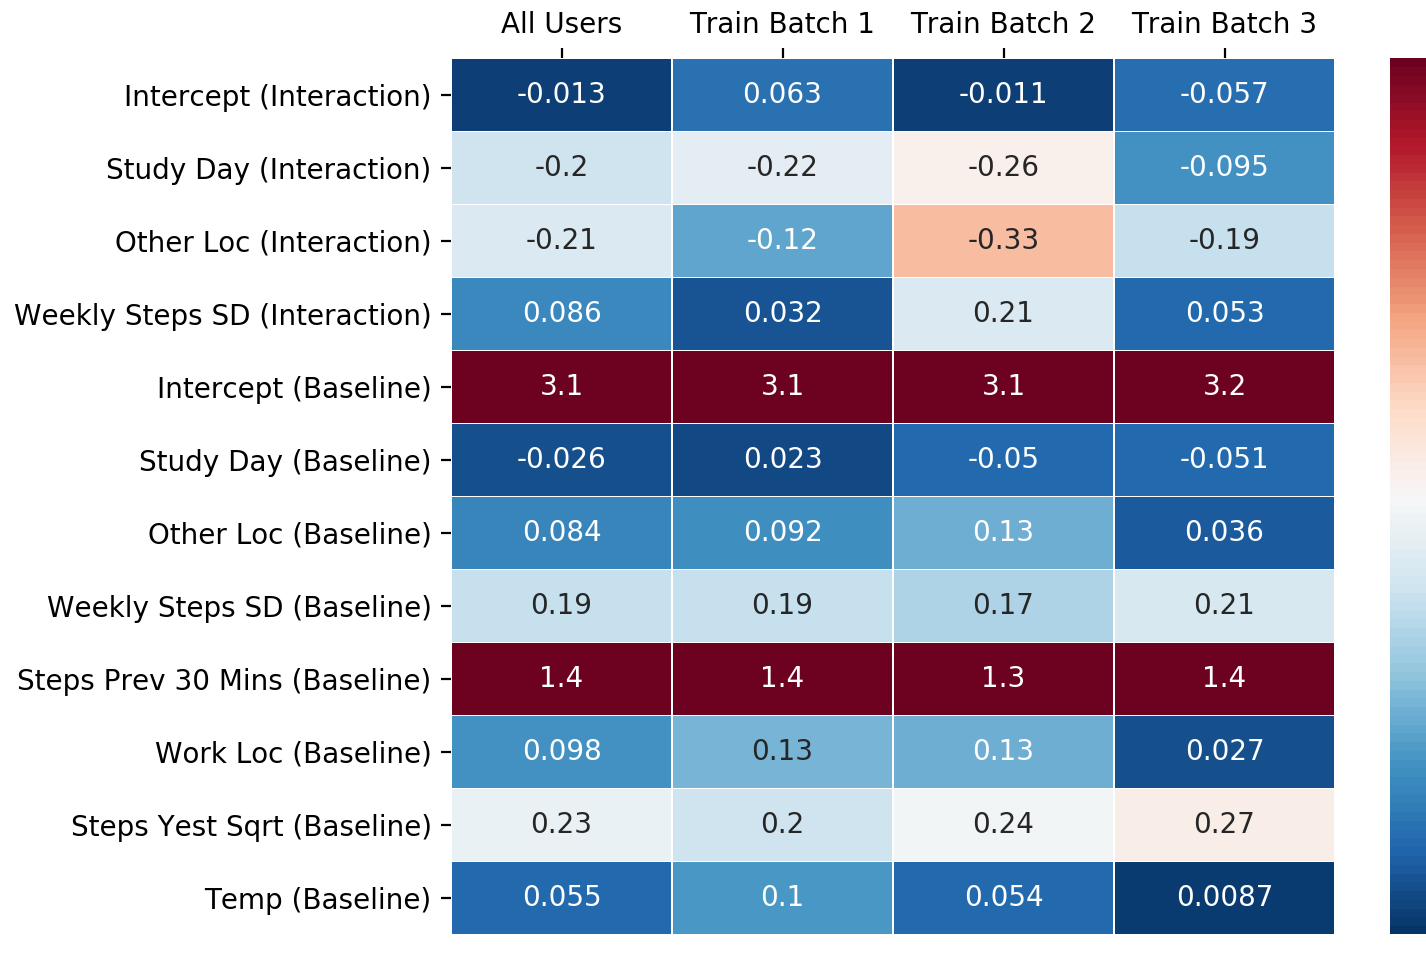
\includegraphics[width=\textwidth]{figures/full_model_coefs_table.png}
\begin{tabular}{rl|rrrr}
\toprule
Feature & {} &  All Users &  Train Batch 1 &  Train Batch 2 &  Train Batch 3 \\
\midrule
Intercept & Interact       &  -0.012933 &       0.063370 &      -0.011041 &      -0.057476 \\
Study Day & Interact       &  -0.199678 &      -0.220172 &      -0.263731 &      -0.095406 \\
Other Loc & Interact       &  -0.212436 &      -0.115700 &      -0.327226 &      -0.191645 \\
Weekly Steps SD & Interact &   0.086211 &       0.031911 &       0.212389 &       0.052531 \\
\hline
Intercept & Baseline          &   3.128955 &       3.097138 &       3.112697 &       3.182046 \\
Study Day & Baseline          &  -0.026399 &       0.023134 &      -0.050334 &      -0.051322 \\
Other Loc & Baseline          &   0.084443 &       0.092011 &       0.128750 &       0.035890 \\
Weekly Steps SD & Baseline    &   0.190982 &       0.192708 &       0.172558 &       0.205276 \\
Steps Prev 30 Mins & Baseline &   1.364978 &       1.352779 &       1.336849 &       1.400528 \\
Work Loc & Baseline           &   0.098259 &       0.131462 &       0.128784 &       0.026610 \\
Steps Yest Sqrt & Baseline    &   0.231959 &       0.198348 &       0.243200 &       0.269906 \\
Temp & Baseline               &   0.054507 &       0.101924 &       0.053583 &       0.008715 \\
\bottomrule
\end{tabular}

\caption{Full Model Regression $\hat{\Theta}$ Estimates}
\end{figure}

\begin{table}
\begin{tabular}{lclc}
\toprule
\textbf{Dep. Variable:}                &      Reward       & \textbf{  R-squared:         } &     0.237   \\
\textbf{Model:}                        &       OLS        & \textbf{  Adj. R-squared:    } &     0.236   \\
\textbf{Method:}                       &  Least Squares   & \textbf{  F-statistic:       } &     168.1   \\
\textbf{Date:}                         & Sat, 05 May 2018 & \textbf{  Prob (F-statistic):} &     0.00    \\
\textbf{Time:}                         &     22:47:56     & \textbf{  Log-Likelihood:    } &   -14307.   \\
\textbf{No. Observations:}             &        5961      & \textbf{  AIC:               } & 2.864e+04   \\
\textbf{Df Residuals:}                 &        5949      & \textbf{  BIC:               } & 2.872e+04   \\
\textbf{Df Model:}                     &          11      & \textbf{                     } &             \\
\bottomrule
\end{tabular}
\begin{tabular}{lcccccc}
                                       & \textbf{coef} & \textbf{std err} & \textbf{t} & \textbf{P$>$$|$t$|$} & \textbf{[0.025} & \textbf{0.975]}  \\
\midrule
\textbf{Intercept (Interaction)}       &      -0.0129  &        0.074     &    -0.174  &         0.862        &       -0.158    &        0.133     \\
\textbf{Study Day (Interaction)}       &      -0.1997  &        0.074     &    -2.708  &         0.007        &       -0.344    &       -0.055     \\
\textbf{Other Loc (Interaction)}       &      -0.2124  &        0.073     &    -2.925  &         0.003        &       -0.355    &       -0.070     \\
\textbf{Weekly Steps SD (Interaction)} &       0.0862  &        0.082     &     1.053  &         0.292        &       -0.074    &        0.247     \\
\textbf{Intercept (Baseline)}          &       3.1290  &        0.043     &    73.188  &         0.000        &        3.045    &        3.213     \\
\textbf{Study Day (Baseline)}          &      -0.0264  &        0.043     &    -0.610  &         0.542        &       -0.111    &        0.058     \\
\textbf{Other Loc (Baseline)}          &       0.0844  &        0.049     &     1.712  &         0.087        &       -0.012    &        0.181     \\
\textbf{Weekly Steps SD (Baseline)}    &       0.1910  &        0.048     &     4.009  &         0.000        &        0.098    &        0.284     \\
\textbf{Steps Prev 30 Mins (Baseline)} &       1.3650  &        0.035     &    38.626  &         0.000        &        1.296    &        1.434     \\
\textbf{Work Loc (Baseline)}           &       0.0983  &        0.041     &     2.392  &         0.017        &        0.018    &        0.179     \\
\textbf{Steps Yest Sqrt (Baseline)}    &       0.2320  &        0.036     &     6.390  &         0.000        &        0.161    &        0.303     \\
\textbf{Temp (Baseline)}               &       0.0545  &        0.038     &     1.428  &         0.153        &       -0.020    &        0.129     \\
\bottomrule
\end{tabular}
\begin{tabular}{lclc}
\textbf{Omnibus:}       & 281.851 & \textbf{  Durbin-Watson:     } &    1.915  \\
\textbf{Prob(Omnibus):} &   0.000 & \textbf{  Jarque-Bera (JB):  } &  150.891  \\
\textbf{Skew:}          &  -0.223 & \textbf{  Prob(JB):          } & 1.72e-33  \\
\textbf{Kurtosis:}      &   2.360 & \textbf{  Cond. No.          } &     3.34  \\
\bottomrule
\end{tabular}
\caption{Full Model Regression, All Users Together}
\end{table}

\medskip

\begin{table}
\begin{tabular}{lclc}
\toprule
\textbf{Dep. Variable:}                &      Reward       & \textbf{  R-squared:         } &     0.231   \\
\textbf{Model:}                        &       OLS        & \textbf{  Adj. R-squared:    } &     0.229   \\
\textbf{Method:}                       &  Least Squares   & \textbf{  F-statistic:       } &     108.6   \\
\textbf{Date:}                         & Sat, 05 May 2018 & \textbf{  Prob (F-statistic):} & 3.07e-217   \\
\textbf{Time:}                         &     22:47:56     & \textbf{  Log-Likelihood:    } &   -9619.4   \\
\textbf{No. Observations:}             &        3983      & \textbf{  AIC:               } & 1.926e+04   \\
\textbf{Df Residuals:}                 &        3971      & \textbf{  BIC:               } & 1.934e+04   \\
\textbf{Df Model:}                     &          11      & \textbf{                     } &             \\
\bottomrule
\end{tabular}
\begin{tabular}{lcccccc}
                                       & \textbf{coef} & \textbf{std err} & \textbf{t} & \textbf{P$>$$|$t$|$} & \textbf{[0.025} & \textbf{0.975]}  \\
\midrule
\textbf{Intercept (Interaction)}       &       0.0634  &        0.094     &     0.673  &         0.501        &       -0.121    &        0.248     \\
\textbf{Study Day (Interaction)}       &      -0.2202  &        0.092     &    -2.381  &         0.017        &       -0.401    &       -0.039     \\
\textbf{Other Loc (Interaction)}       &      -0.1157  &        0.089     &    -1.297  &         0.195        &       -0.291    &        0.059     \\
\textbf{Weekly Steps SD (Interaction)} &       0.0319  &        0.090     &     0.354  &         0.723        &       -0.145    &        0.209     \\
\textbf{Intercept (Baseline)}          &       3.0971  &        0.053     &    58.455  &         0.000        &        2.993    &        3.201     \\
\textbf{Study Day (Baseline)}          &       0.0231  &        0.054     &     0.431  &         0.666        &       -0.082    &        0.128     \\
\textbf{Other Loc (Baseline)}          &       0.0920  &        0.059     &     1.572  &         0.116        &       -0.023    &        0.207     \\
\textbf{Weekly Steps SD (Baseline)}    &       0.1927  &        0.052     &     3.703  &         0.000        &        0.091    &        0.295     \\
\textbf{Steps Prev 30 Mins (Baseline)} &       1.3528  &        0.044     &    30.987  &         0.000        &        1.267    &        1.438     \\
\textbf{Work Loc (Baseline)}           &       0.1315  &        0.050     &     2.635  &         0.008        &        0.034    &        0.229     \\
\textbf{Steps Yest Sqrt (Baseline)}    &       0.1983  &        0.043     &     4.627  &         0.000        &        0.114    &        0.282     \\
\textbf{Temp (Baseline)}               &       0.1019  &        0.048     &     2.110  &         0.035        &        0.007    &        0.197     \\
\bottomrule
\end{tabular}
\begin{tabular}{lclc}
\textbf{Omnibus:}       & 197.556 & \textbf{  Durbin-Watson:     } &    1.882  \\
\textbf{Prob(Omnibus):} &   0.000 & \textbf{  Jarque-Bera (JB):  } &   97.931  \\
\textbf{Skew:}          &  -0.196 & \textbf{  Prob(JB):          } & 5.43e-22  \\
\textbf{Kurtosis:}      &   2.339 & \textbf{  Cond. No.          } &     3.31  \\
\bottomrule
\end{tabular}
\caption{Full Model Regression, Training Batch 1}
\end{table}

\medskip

\begin{table}
\begin{tabular}{lclc}
\toprule
\textbf{Dep. Variable:}                &      Reward       & \textbf{  R-squared:         } &     0.236   \\
\textbf{Model:}                        &       OLS        & \textbf{  Adj. R-squared:    } &     0.234   \\
\textbf{Method:}                       &  Least Squares   & \textbf{  F-statistic:       } &     113.5   \\
\textbf{Date:}                         & Sat, 05 May 2018 & \textbf{  Prob (F-statistic):} & 1.31e-226   \\
\textbf{Time:}                         &     22:47:56     & \textbf{  Log-Likelihood:    } &   -9754.8   \\
\textbf{No. Observations:}             &        4057      & \textbf{  AIC:               } & 1.953e+04   \\
\textbf{Df Residuals:}                 &        4045      & \textbf{  BIC:               } & 1.961e+04   \\
\textbf{Df Model:}                     &          11      & \textbf{                     } &             \\
\bottomrule
\end{tabular}
\begin{tabular}{lcccccc}
                                       & \textbf{coef} & \textbf{std err} & \textbf{t} & \textbf{P$>$$|$t$|$} & \textbf{[0.025} & \textbf{0.975]}  \\
\midrule
\textbf{Intercept (Interaction)}       &      -0.0110  &        0.089     &    -0.124  &         0.902        &       -0.186    &        0.164     \\
\textbf{Study Day (Interaction)}       &      -0.2637  &        0.089     &    -2.960  &         0.003        &       -0.438    &       -0.089     \\
\textbf{Other Loc (Interaction)}       &      -0.3272  &        0.090     &    -3.638  &         0.000        &       -0.504    &       -0.151     \\
\textbf{Weekly Steps SD (Interaction)} &       0.2124  &        0.116     &     1.838  &         0.066        &       -0.014    &        0.439     \\
\textbf{Intercept (Baseline)}          &       3.1127  &        0.053     &    58.396  &         0.000        &        3.008    &        3.217     \\
\textbf{Study Day (Baseline)}          &      -0.0503  &        0.053     &    -0.948  &         0.343        &       -0.154    &        0.054     \\
\textbf{Other Loc (Baseline)}          &       0.1288  &        0.065     &     1.975  &         0.048        &        0.001    &        0.257     \\
\textbf{Weekly Steps SD (Baseline)}    &       0.1726  &        0.071     &     2.433  &         0.015        &        0.034    &        0.312     \\
\textbf{Steps Prev 30 Mins (Baseline)} &       1.3368  &        0.043     &    31.015  &         0.000        &        1.252    &        1.421     \\
\textbf{Work Loc (Baseline)}           &       0.1288  &        0.051     &     2.517  &         0.012        &        0.028    &        0.229     \\
\textbf{Steps Yest Sqrt (Baseline)}    &       0.2432  &        0.046     &     5.291  &         0.000        &        0.153    &        0.333     \\
\textbf{Temp (Baseline)}               &       0.0536  &        0.047     &     1.140  &         0.254        &       -0.039    &        0.146     \\
\bottomrule
\end{tabular}
\begin{tabular}{lclc}
\textbf{Omnibus:}       & 240.090 & \textbf{  Durbin-Watson:     } &    1.917  \\
\textbf{Prob(Omnibus):} &   0.000 & \textbf{  Jarque-Bera (JB):  } &  110.868  \\
\textbf{Skew:}          &  -0.203 & \textbf{  Prob(JB):          } & 8.42e-25  \\
\textbf{Kurtosis:}      &   2.300 & \textbf{  Cond. No.          } &     4.04  \\
\bottomrule
\end{tabular}
\caption{Full Model Regression, Training Batch 2}
\end{table}

\medskip

\begin{table}
\begin{tabular}{lclc}
\toprule
\textbf{Dep. Variable:}                &      Reward       & \textbf{  R-squared:         } &     0.248   \\
\textbf{Model:}                        &       OLS        & \textbf{  Adj. R-squared:    } &     0.246   \\
\textbf{Method:}                       &  Least Squares   & \textbf{  F-statistic:       } &     116.1   \\
\textbf{Date:}                         & Sat, 05 May 2018 & \textbf{  Prob (F-statistic):} & 4.65e-230   \\
\textbf{Time:}                         &     22:47:56     & \textbf{  Log-Likelihood:    } &   -9227.7   \\
\textbf{No. Observations:}             &        3882      & \textbf{  AIC:               } & 1.848e+04   \\
\textbf{Df Residuals:}                 &        3870      & \textbf{  BIC:               } & 1.855e+04   \\
\textbf{Df Model:}                     &          11      & \textbf{                     } &             \\
\bottomrule
\end{tabular}
\begin{tabular}{lcccccc}
                                       & \textbf{coef} & \textbf{std err} & \textbf{t} & \textbf{P$>$$|$t$|$} & \textbf{[0.025} & \textbf{0.975]}  \\
\midrule
\textbf{Intercept (Interaction)}       &      -0.0575  &        0.091     &    -0.634  &         0.526        &       -0.235    &        0.120     \\
\textbf{Study Day (Interaction)}       &      -0.0954  &        0.090     &    -1.066  &         0.287        &       -0.271    &        0.080     \\
\textbf{Other Loc (Interaction)}       &      -0.1916  &        0.088     &    -2.170  &         0.030        &       -0.365    &       -0.018     \\
\textbf{Weekly Steps SD (Interaction)} &       0.0525  &        0.101     &     0.519  &         0.604        &       -0.146    &        0.251     \\
\textbf{Intercept (Baseline)}          &       3.1820  &        0.052     &    60.638  &         0.000        &        3.079    &        3.285     \\
\textbf{Study Day (Baseline)}          &      -0.0513  &        0.052     &    -0.981  &         0.327        &       -0.154    &        0.051     \\
\textbf{Other Loc (Baseline)}          &       0.0359  &        0.059     &     0.610  &         0.542        &       -0.080    &        0.151     \\
\textbf{Weekly Steps SD (Baseline)}    &       0.2053  &        0.057     &     3.605  &         0.000        &        0.094    &        0.317     \\
\textbf{Steps Prev 30 Mins (Baseline)} &       1.4005  &        0.043     &    32.403  &         0.000        &        1.316    &        1.485     \\
\textbf{Work Loc (Baseline)}           &       0.0266  &        0.052     &     0.514  &         0.607        &       -0.075    &        0.128     \\
\textbf{Steps Yest Sqrt (Baseline)}    &       0.2699  &        0.045     &     5.978  &         0.000        &        0.181    &        0.358     \\
\textbf{Temp (Baseline)}               &       0.0087  &        0.047     &     0.186  &         0.852        &       -0.083    &        0.100     \\
\bottomrule
\end{tabular}
\begin{tabular}{lclc}
\textbf{Omnibus:}       & 141.111 & \textbf{  Durbin-Watson:     } &    1.962  \\
\textbf{Prob(Omnibus):} &   0.000 & \textbf{  Jarque-Bera (JB):  } &   95.075  \\
\textbf{Skew:}          &  -0.267 & \textbf{  Prob(JB):          } & 2.26e-21  \\
\textbf{Kurtosis:}      &   2.450 & \textbf{  Cond. No.          } &     3.32  \\
\bottomrule
\end{tabular}
\caption{Full Model Regression, Training Batch 3}
\end{table}

\medskip



%%%%%%%%%%%%%%%%%%%%%%%%%%%%%%%%%%%%%%%%%%%%%%%%%%%%
\section{Small Model OLS Results}


\begin{figure}
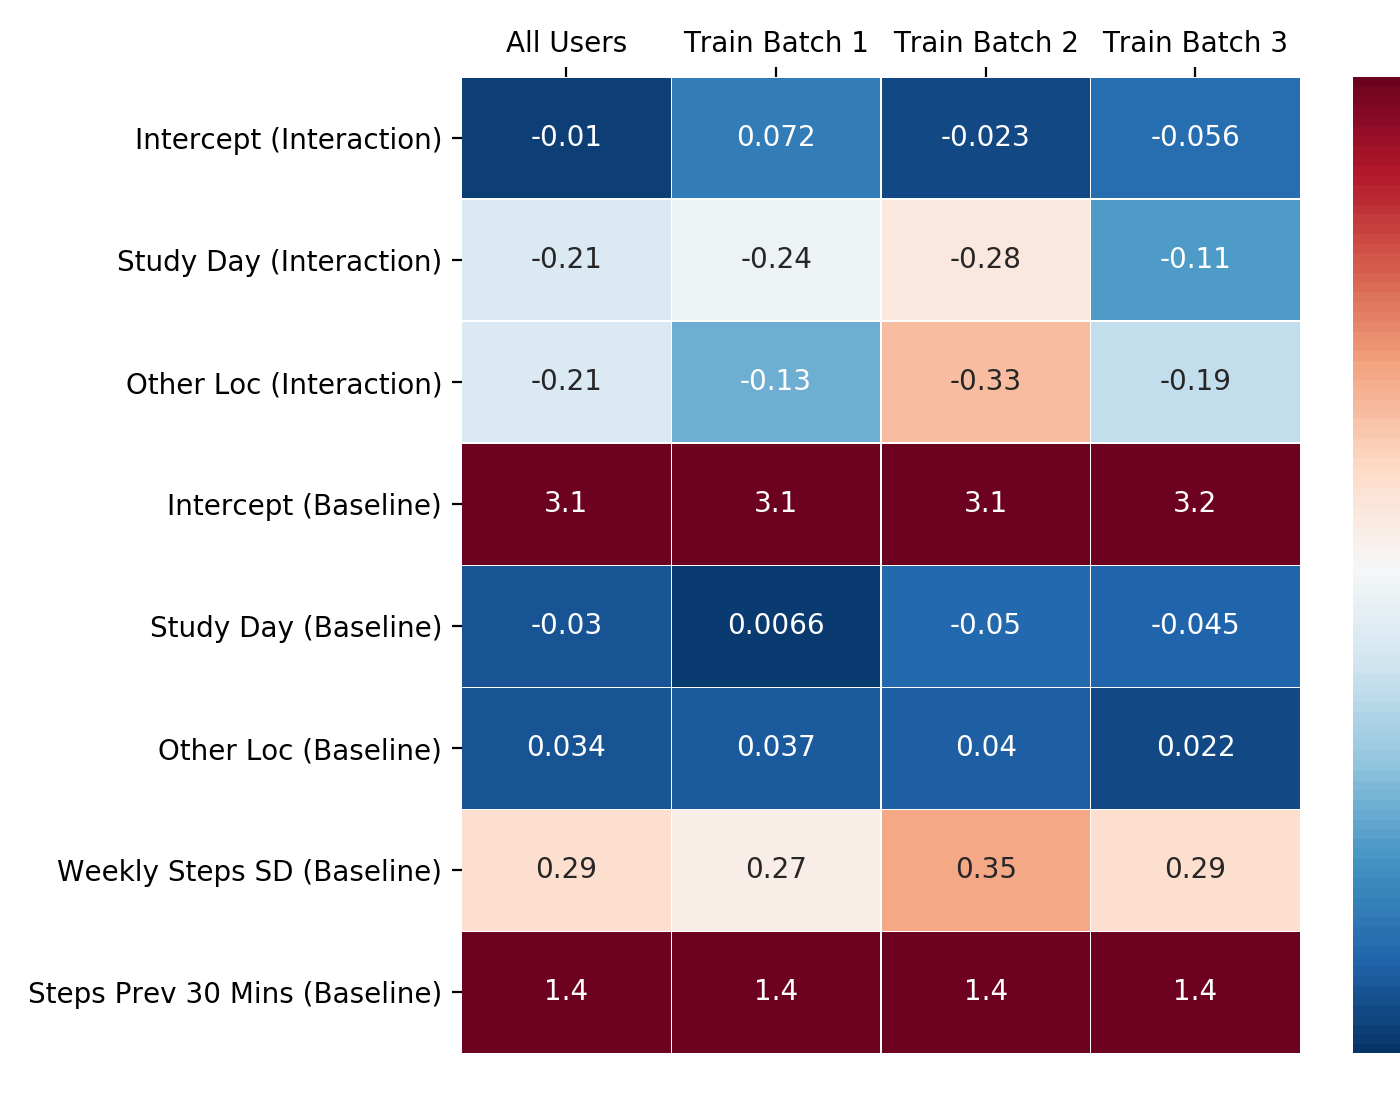
\includegraphics[width=\textwidth]{figures/small_model_coefs_table.png}
\begin{tabular}{rl|rrrr}
\toprule
Feature & {} & All Users &  Train Batch 1 &  Train Batch 2 &  Train Batch 3 \\
\midrule
Intercept & Interact       &  -0.010436 &       0.071858 &      -0.023353 &      -0.056086 \\
Study Day & Interact       &  -0.211407 &      -0.236143 &      -0.276794 &      -0.107167 \\
Other Loc & Interact       &  -0.214480 &      -0.125237 &      -0.325202 &      -0.185378 \\
\hline
Intercept & Baseline          &   3.127301 &       3.096886 &       3.125608 &       3.163705 \\
Study Day & Baseline          &  -0.030159 &       0.006554 &      -0.050069 &      -0.045362 \\
Other Loc & Baseline          &   0.033786 &       0.037067 &       0.040477 &       0.022279 \\
Weekly Steps SD & Baseline    &   0.292857 &       0.266203 &       0.347553 &       0.290910 \\
Steps Prev 30 Mins & Baseline &   1.384952 &       1.370012 &       1.358397 &       1.425091 \\
\bottomrule
\end{tabular}


\caption{Small Model Regression $\hat{\Theta}$ Estimates}
\end{figure}


\begin{table}
\begin{tabular}{lclc}
\toprule
\textbf{Dep. Variable:}                &      Reward       & \textbf{  R-squared:         } &     0.230   \\
\textbf{Model:}                        &       OLS        & \textbf{  Adj. R-squared:    } &     0.230   \\
\textbf{Method:}                       &  Least Squares   & \textbf{  F-statistic:       } &     254.6   \\
\textbf{Date:}                         & Sat, 05 May 2018 & \textbf{  Prob (F-statistic):} &     0.00    \\
\textbf{Time:}                         &     22:46:55     & \textbf{  Log-Likelihood:    } &   -14334.   \\
\textbf{No. Observations:}             &        5961      & \textbf{  AIC:               } & 2.868e+04   \\
\textbf{Df Residuals:}                 &        5953      & \textbf{  BIC:               } & 2.874e+04   \\
\textbf{Df Model:}                     &           7      & \textbf{                     } &             \\
\bottomrule
\end{tabular}
\begin{tabular}{lcccccc}
                                       & \textbf{coef} & \textbf{std err} & \textbf{t} & \textbf{P$>$$|$t$|$} & \textbf{[0.025} & \textbf{0.975]}  \\
\midrule
\textbf{Intercept (Interaction)}       &      -0.0104  &        0.074     &    -0.140  &         0.889        &       -0.156    &        0.136     \\
\textbf{Study Day (Interaction)}       &      -0.2114  &        0.074     &    -2.863  &         0.004        &       -0.356    &       -0.067     \\
\textbf{Other Loc (Interaction)}       &      -0.2145  &        0.073     &    -2.943  &         0.003        &       -0.357    &       -0.072     \\
\textbf{Intercept (Baseline)}          &       3.1273  &        0.043     &    72.859  &         0.000        &        3.043    &        3.211     \\
\textbf{Study Day (Baseline)}          &      -0.0302  &        0.043     &    -0.703  &         0.482        &       -0.114    &        0.054     \\
\textbf{Other Loc (Baseline)}          &       0.0338  &        0.045     &     0.757  &         0.449        &       -0.054    &        0.121     \\
\textbf{Weekly Steps SD (Baseline)}    &       0.2929  &        0.039     &     7.588  &         0.000        &        0.217    &        0.369     \\
\textbf{Steps Prev 30 Mins (Baseline)} &       1.3850  &        0.035     &    39.227  &         0.000        &        1.316    &        1.454     \\
\bottomrule
\end{tabular}
\begin{tabular}{lclc}
\textbf{Omnibus:}       & 294.145 & \textbf{  Durbin-Watson:     } &    1.896  \\
\textbf{Prob(Omnibus):} &   0.000 & \textbf{  Jarque-Bera (JB):  } &  144.932  \\
\textbf{Skew:}          &  -0.192 & \textbf{  Prob(JB):          } & 3.38e-32  \\
\textbf{Kurtosis:}      &   2.340 & \textbf{  Cond. No.          } &     2.73  \\
\bottomrule
\end{tabular}
\caption{Small Model Regression, All Users Together}
\end{table}

\medskip

\begin{table}
\begin{tabular}{lclc}
\toprule
\textbf{Dep. Variable:}                &      Reward       & \textbf{  R-squared:         } &     0.225   \\
\textbf{Model:}                        &       OLS        & \textbf{  Adj. R-squared:    } &     0.223   \\
\textbf{Method:}                       &  Least Squares   & \textbf{  F-statistic:       } &     164.7   \\
\textbf{Date:}                         & Sat, 05 May 2018 & \textbf{  Prob (F-statistic):} & 2.13e-214   \\
\textbf{Time:}                         &     22:46:55     & \textbf{  Log-Likelihood:    } &   -9636.0   \\
\textbf{No. Observations:}             &        3983      & \textbf{  AIC:               } & 1.929e+04   \\
\textbf{Df Residuals:}                 &        3975      & \textbf{  BIC:               } & 1.934e+04   \\
\textbf{Df Model:}                     &           7      & \textbf{                     } &             \\
\bottomrule
\end{tabular}
\begin{tabular}{lcccccc}
                                       & \textbf{coef} & \textbf{std err} & \textbf{t} & \textbf{P$>$$|$t$|$} & \textbf{[0.025} & \textbf{0.975]}  \\
\midrule
\textbf{Intercept (Interaction)}       &       0.0719  &        0.094     &     0.763  &         0.446        &       -0.113    &        0.257     \\
\textbf{Study Day (Interaction)}       &      -0.2361  &        0.093     &    -2.551  &         0.011        &       -0.418    &       -0.055     \\
\textbf{Other Loc (Interaction)}       &      -0.1252  &        0.089     &    -1.400  &         0.162        &       -0.301    &        0.050     \\
\textbf{Intercept (Baseline)}          &       3.0969  &        0.053     &    58.427  &         0.000        &        2.993    &        3.201     \\
\textbf{Study Day (Baseline)}          &       0.0066  &        0.053     &     0.124  &         0.902        &       -0.097    &        0.111     \\
\textbf{Other Loc (Baseline)}          &       0.0371  &        0.054     &     0.685  &         0.493        &       -0.069    &        0.143     \\
\textbf{Weekly Steps SD (Baseline)}    &       0.2662  &        0.042     &     6.293  &         0.000        &        0.183    &        0.349     \\
\textbf{Steps Prev 30 Mins (Baseline)} &       1.3700  &        0.044     &    31.476  &         0.000        &        1.285    &        1.455     \\
\bottomrule
\end{tabular}
\begin{tabular}{lclc}
\textbf{Omnibus:}       & 206.934 & \textbf{  Durbin-Watson:     } &    1.867  \\
\textbf{Prob(Omnibus):} &   0.000 & \textbf{  Jarque-Bera (JB):  } &   95.047  \\
\textbf{Skew:}          &  -0.167 & \textbf{  Prob(JB):          } & 2.30e-21  \\
\textbf{Kurtosis:}      &   2.321 & \textbf{  Cond. No.          } &     2.89  \\
\bottomrule
\end{tabular}
\caption{Small Model Regression, Training Batch 1}
\end{table}

\medskip

\begin{table}
\begin{tabular}{lclc}
\toprule
\textbf{Dep. Variable:}                &      Reward       & \textbf{  R-squared:         } &     0.228   \\
\textbf{Model:}                        &       OLS        & \textbf{  Adj. R-squared:    } &     0.227   \\
\textbf{Method:}                       &  Least Squares   & \textbf{  F-statistic:       } &     170.7   \\
\textbf{Date:}                         & Sat, 05 May 2018 & \textbf{  Prob (F-statistic):} & 6.01e-222   \\
\textbf{Time:}                         &     22:46:55     & \textbf{  Log-Likelihood:    } &   -9775.8   \\
\textbf{No. Observations:}             &        4057      & \textbf{  AIC:               } & 1.957e+04   \\
\textbf{Df Residuals:}                 &        4049      & \textbf{  BIC:               } & 1.962e+04   \\
\textbf{Df Model:}                     &           7      & \textbf{                     } &             \\
\bottomrule
\end{tabular}
\begin{tabular}{lcccccc}
                                       & \textbf{coef} & \textbf{std err} & \textbf{t} & \textbf{P$>$$|$t$|$} & \textbf{[0.025} & \textbf{0.975]}  \\
\midrule
\textbf{Intercept (Interaction)}       &      -0.0234  &        0.090     &    -0.261  &         0.794        &       -0.199    &        0.152     \\
\textbf{Study Day (Interaction)}       &      -0.2768  &        0.089     &    -3.104  &         0.002        &       -0.452    &       -0.102     \\
\textbf{Other Loc (Interaction)}       &      -0.3252  &        0.090     &    -3.601  &         0.000        &       -0.502    &       -0.148     \\
\textbf{Intercept (Baseline)}          &       3.1256  &        0.053     &    58.908  &         0.000        &        3.022    &        3.230     \\
\textbf{Study Day (Baseline)}          &      -0.0501  &        0.053     &    -0.950  &         0.342        &       -0.153    &        0.053     \\
\textbf{Other Loc (Baseline)}          &       0.0405  &        0.056     &     0.723  &         0.470        &       -0.069    &        0.150     \\
\textbf{Weekly Steps SD (Baseline)}    &       0.3476  &        0.056     &     6.210  &         0.000        &        0.238    &        0.457     \\
\textbf{Steps Prev 30 Mins (Baseline)} &       1.3584  &        0.043     &    31.485  &         0.000        &        1.274    &        1.443     \\
\bottomrule
\end{tabular}
\begin{tabular}{lclc}
\textbf{Omnibus:}       & 248.433 & \textbf{  Durbin-Watson:     } &    1.900  \\
\textbf{Prob(Omnibus):} &   0.000 & \textbf{  Jarque-Bera (JB):  } &  106.236  \\
\textbf{Skew:}          &  -0.170 & \textbf{  Prob(JB):          } & 8.53e-24  \\
\textbf{Kurtosis:}      &   2.284 & \textbf{  Cond. No.          } &     2.74  \\
\bottomrule
\end{tabular}
\caption{Small Model Regression, Training Batch 2}
\end{table}

\medskip

\begin{table}
\begin{tabular}{lclc}
\toprule
\textbf{Dep. Variable:}                &      Reward       & \textbf{  R-squared:         } &     0.241   \\
\textbf{Model:}                        &       OLS        & \textbf{  Adj. R-squared:    } &     0.240   \\
\textbf{Method:}                       &  Least Squares   & \textbf{  F-statistic:       } &     175.7   \\
\textbf{Date:}                         & Sat, 05 May 2018 & \textbf{  Prob (F-statistic):} & 1.80e-226   \\
\textbf{Time:}                         &     22:46:55     & \textbf{  Log-Likelihood:    } &   -9246.3   \\
\textbf{No. Observations:}             &        3882      & \textbf{  AIC:               } & 1.851e+04   \\
\textbf{Df Residuals:}                 &        3874      & \textbf{  BIC:               } & 1.856e+04   \\
\textbf{Df Model:}                     &           7      & \textbf{                     } &             \\
\bottomrule
\end{tabular}
\begin{tabular}{lcccccc}
                                       & \textbf{coef} & \textbf{std err} & \textbf{t} & \textbf{P$>$$|$t$|$} & \textbf{[0.025} & \textbf{0.975]}  \\
\midrule
\textbf{Intercept (Interaction)}       &      -0.0561  &        0.091     &    -0.618  &         0.537        &       -0.234    &        0.122     \\
\textbf{Study Day (Interaction)}       &      -0.1072  &        0.090     &    -1.196  &         0.232        &       -0.283    &        0.069     \\
\textbf{Other Loc (Interaction)}       &      -0.1854  &        0.089     &    -2.091  &         0.037        &       -0.359    &       -0.012     \\
\textbf{Intercept (Baseline)}          &       3.1637  &        0.052     &    60.819  &         0.000        &        3.062    &        3.266     \\
\textbf{Study Day (Baseline)}          &      -0.0454  &        0.052     &    -0.873  &         0.383        &       -0.147    &        0.056     \\
\textbf{Other Loc (Baseline)}          &       0.0223  &        0.054     &     0.412  &         0.681        &       -0.084    &        0.128     \\
\textbf{Weekly Steps SD (Baseline)}    &       0.2909  &        0.047     &     6.210  &         0.000        &        0.199    &        0.383     \\
\textbf{Steps Prev 30 Mins (Baseline)} &       1.4251  &        0.043     &    33.022  &         0.000        &        1.340    &        1.510     \\
\bottomrule
\end{tabular}
\begin{tabular}{lclc}
\textbf{Omnibus:}       & 146.229 & \textbf{  Durbin-Watson:     } &    1	.936  \\
\textbf{Prob(Omnibus):} &   0.000 & \textbf{  Jarque-Bera (JB):  } &   92.085  \\
\textbf{Skew:}          &  -0.246 & \textbf{  Prob(JB):          } & 1.01e-20  \\
\textbf{Kurtosis:}      &   2.428 & \textbf{  Cond. No.          } &     2.73  \\
\bottomrule
\end{tabular}
\caption{Small Model Regression, Training Batch 3}
\end{table}

\medskip
